\documentclass[conference]{IEEEtran}
\IEEEoverridecommandlockouts
% The preceding line is only needed to identify funding in the first footnote. If that is unneeded, please comment it out.
\usepackage{cite}
\usepackage{amsmath,amssymb,amsfonts}
\usepackage{algorithmic}
\usepackage{graphicx}
\usepackage{textcomp}
\usepackage{xcolor}
\def\BibTeX{{\rm B\kern-.05em{\sc i\kern-.025em b}\kern-.08em
    T\kern-.1667em\lower.7ex\hbox{E}\kern-.125emX}}
\begin{document}
\bibliographystyle{plain}

\title{Adaptation and Learning Neurally}

\author{\IEEEauthorblockN{Giulio Pace}
\IEEEauthorblockA{\textit{TUWien} \\
\textit{11835706}\\
Vienna, Austria \\
giulio.pace93@gmail.com}
\and
\IEEEauthorblockN{David Penz}
\IEEEauthorblockA{\textit{TUWien} \\
\textit{11703497}\\
Vienna, Austria \\
e11703497@student.tuwien.ac.at}
}

\maketitle

\begin{abstract}
	Adaptation and Learning are fundamental processes of the human brain. Adaptation is an unconscious process that every species needs in order to survive to the wide range of different stimuli provided by the world. Learning is the process of acquiring new information and storing it for future usage, both consciously and unconsciously. In this paper we will explain these concepts in detail and show how they both lie for the most part on the unconscious side of our mind.
\end{abstract}

\begin{IEEEkeywords}
	Adaptation, Learning, Neurally, Consciousness model, Neural Network.
\end{IEEEkeywords}

\section{Introduction}

	Adaptation and learning are key concepts in the development and growth of humans and non-humans. In the 1990s, G. M. Stratton conducted a series of experiments to gain insights and further prove the theory of adaptation. One specific experiment was about the effects of wearing a pair of glasses for eight days, which flipped the visual perception of his environment, i.e. the glasses inverted the images received by the retina upside down. On day five, G. M. Stratton was able to perceive his surroundings as he would see it without the inverting glasses as his brain was able to undo the changes caused by them, although, he could still see the images inverted by concentrating. From that experiment, he concluded that the human brain is able to adapt to changes. \cite{a1}

	The process of learning and adaptation is present throughout the whole lifespan of a human or non-human. An individual has to learn several skills and adapt to a variety of changes and stimuli such as:
	\begin{itemize}
		\item Learn how to walk as an infant;
		\item Learn how to communicate with other individuals;
		\item Learn how to hunt for food;
		\item Adapt to climate changes;
		\item Adapt to feedback gained from experience or other individuals.
	\end{itemize}

	As seen in the above described examples, learning and adaptation tackle different types of problems coming with their own challenges each. Also, there are different ways of looking at how learning and adapting to changes might work, e.g. learning can be defined in the field of psychology but could also be described in a neurological environment.

	This paper aims to create an understanding of what learning and adaptation might be defined as in different disciplines of areas. In order to do so, the first three chapters will look at and compare different scientific literature in:

	\begin{itemize}
		\item Psychology
		\item Neurology
		\item Learning Theory
		\item Educational Studies
		\item Linguistics
		\item Computer Science
	\end{itemize}
	We will further expand how the topic is used in the field of Computer Science in chapter VI, where we will explore how neural networks are linked to Adaptation and Learning and how these concepts are key to understand the lastest Deep Learning advancements.
	Furthermore, we want to identify possible connections to a consciousness model that we will cover in chapter V, showing that both Adaptation and Learning are part of the lower and less conscious part of our brain.

\section{Adaptation and Learning in the psychological literature}

	In this chapter we will focus on comparing different definitions of the terms “learning” and “adaptation” within existing literature and papers in the psychological science field. The goal is to create an overview of possible definitions by looking at similarities as well as differences.

	At first, we will take a look at the term “adaptation”. In their publication “Evaluating Evidence of Psychological Adaptation: How Do We Know One When We See One?” \cite{b1}, David P. Schmitt and June J. Pilcher refer to adaptation as both, a verb and a noun:
	\begin{itemize}
		\item Adaptation as a verb defines the process of evolution, where an animal (human or non-human) will change either on an individual basis or over the lifespan of its species to overcome challenges in its environment and become better suited to survive in the given environment;
		\item Adaptation as a noun defines the outcome or product of evolution, where they further narrow it down to two basic forms. On the one side, adaptation might be seen as a characteristic feature of an animal in order to survive or reproduce in its given environment, on the other hand, it can also be defined as the “historical end products of the process of evolution”.
	\end{itemize}

	The term “learning” can be seen similarly to the term “adaptation”. G. Hall defines the act of learning in \cite{b2} as the process by which a creature “interacts with its environment and becomes changed by this experience so that its subsequent behaviour is modified”. In \cite{b3}, learning is also described as a process of gaining new characteristic features based on study or experience. Linking the process of adapting to changes and learning based on experience, Robert A. Rescorla defines the term “learning” in \cite{b4} as “a process by which an organism benefits from experience so that its future behaviour is better adapted to its environment”.

	Another way of looking at the process of learning in a psychology is to describe it as a change in a creatures' behaviour, similarly to what adaptation as a noun can be seen as. Jan De Houwer describes learning as a set of changes in a creatures' behaviour resulting from patterns in its environment \cite{b5}, resulting from his observations from two other definitions, functionally as “changes in behaviour that result from experience” and mechanistically as “changes in the organism that result from experience”.

	In \cite{b6}, the definition of the term “learning” is also seen as problematic, as it differs within and across disciplines of research. The conducted study reviewed several scientific papers and publications and concluded in a set of classes: (1) learning defined as the processing of information or experience, (2) learning defined as behavioural change and (3) learning defined as changes in behavioural mechanisms.

\section{Adaptation and Learning in neurology}
	We refer at ``learning'' as the process of acquiring new knowledge or modifying the existing one. Knowledge can not only be about notions but also behaviours, skills, value or preferences.\cite{b7}
	``Memory'' is what allow us to store and retrieve the knowledge we gather through the learning process.
	In neurology it is hard to talk about learning without talking about memory and vice versa. In this chapter we will focus on the different kinds of memory and the brain areas responsible for them.

	\subsection{Memory distinction}\label{MD}
		Memory is a general word used for both Short Term Memory and Long Term Memory. We are now going to focus on the latter, because is where we find the mechanism of adaptation overall of learning.
		We distinguish the Long Term Memory in two categories: ``Explicit Memory'' and ``Implicit Memory''.
		The first kind, also referred as ``Declarative memory'',  stores information about facts, things, people and places. In order for the piece of information to be retrieved, we are required an effort.
		The Explicit Memory is further differentiated in two sub-categories: ``Semantic Memory'', that is about general knowledge of facts about the world around us, and Episodic Memory, in charge of storing information regarding a specific time and space.
		For example, the concept of bicycle is delegated to the Semantic Memory, while the Episodic Memory will take care of remembering episodes related to bicycles.
		The Implicit Memory, also called ``Nondeclarative Memory'', is about learning physical acts or other skills that are recalled automatically and without an active thought towards it.
		It is divided in ``Priming'', ``Procedural Memory'', ``Associative Memory'' and ``Non-Associative Memory''.
		\begin{itemize}
			\item Priming is the influence that a stimulus has on subsequent stimuli;
			\item Procedural Memory is the kind of memory used to learn how to perform specific tasks without thinking. Going back to the bicycle example, this kind of memory ensures that, once learned how to ride a bike, we will be able to ride it without thinking;
			\item The Associative Memory regards the creation of a relation between two or more stimuli or between a stimulus and an associated behaviour, as proved by the experiments conducted by Pavlov and Skinner;
			\item The Non-Associative Memory manages the learning of the properties of a specific stimulus. There are two opposite kinds of non-associative learning: Habituation and sensitization:
			\begin{itemize}
				\item Habituation is defined as a decrease in response to a stimulus repeated in time. The stimulus is marked as ``not harmful'' or ``not useful'' so the subject will start to ignore it.
				\item Sensitization is the opposite phenomenon: after an intense or a noxious stimulus, the subject will overreact to similar stimuli in order to protect itself.
			\end{itemize}
		\end{itemize}

	\subsection{Adaptation}\label{Ad}
		Adaptation is a similar concept to Habituation, but if the latter occurs with stimuli that occur periodically, the first is observed when there is a constant and continuous stimulus.
		On the physical level, mammals and other living organisms are constantly monitoring their environment through receptor cells that allow them to receive and process the stimuli. Through a ion flow, positive or negative feedback are sent to the receptors to allow the cells to close or open channel according to the ion flow. \cite{b8}
		It is believed that adaptation could modify the response range of the neurons in order to encode the signals to a more suitable strength. \cite{b9}

	\subsection{Anatomy of the learning process}\label{ALP}
		Learning is a general term that includes two processes in it: ``Explicit Learning'' and ``Implicit Learning''.
		\begin{itemize}
			\item Explicit Learning refers to the of creating Explicit Memories and it occurs in the hippocampus, neo-cortex and amygdala. \cite{b10} The hippocampus is where episodic memories are created and stored and it is a part of the temporal lobe. After some time in the hippocampus, some memories are moved to the neo-cortex as general knowledge. The amygdala is a structure shaped like an almond that is in the temporal lobe, and gives an emotional background to the memory.
			\item Implicit Learning is the process of creating Implicit Memories and rely on basal ganglia and cerebellum. \cite{b11} Basal ganglia is what we use to store Procedural Memories, while the cerebellum is involved in several motor function like coordination.
		\end{itemize}

\section{Adaptation and Learning in other areas of science}

	Aside from psychology and neurology, which could be seen as research areas related to the human and non-human mind and behaviour, there are many different other areas of research where learning and adaptation is one of the major focus topics. In ``Embracing multiple definitions of learning'' \cite{6}, several other research disciplines are listed, containing but not limited to (1) behavioural ecology, (2) evolutionary theory and (3) computer science. In this chapter, we will cover a selection of different research areas related to learning and adaptation.

	\subsection{Learning Theories}\label{LT}
		Talking about learning and adaptation in a broader sense, Linda Harasim describes in her publication “Learning Theory and Online Technologies” \cite{d1} the basic concepts of learning theory. She defines learning theory as the theory about how humans are able to learn and narrows it down to three subfields, originated in the 20th century:
		\begin{itemize}
			\item Behaviorist learning theory
			\item Cognitivist learning theory
			\item Constructivist learning theory
		\end{itemize}

		Additionally, starting with the 21st century, another subfield of learning theory has emerged, the online collaborative learning theory.

	\subsection{Educational Studies}\label{ES}
		Education starts at the early age of an infant, where learning is a major focus in research, e.g. how infants are able to learn about the physical world they live in \cite{d2}. Another research conducted in the area of education is related to the social environment of students and the definition of a professional learning community \cite{d3}. Within the topic of educational studies, scientific research also covers the topic of learning and teaching first language as well as second language, which we will talk about

	\subsection{Linguistics}\label{Li}
		Within the field of linguistics, research on how to acquire the skill to speak a foreign language has emerged as a discipline related to the term learning \cite{d4}. Within this area, scientific research was conducted on second language learning, but is not limited to it. Several publications cover the connection between first language learning and second language learning by comparing different learning strategies used and how well they work in the respective field. Peter Skehan states in his publication ``A Cognitive Approach to Language Learning'' \cite{d5} that there are some learning strategies which might succeed for first language learning but do not necessarily work well for individuals trying to learn a second language. He also mentions that the act of learning a language cannot be simply done by listening to foreign speakers, e.g. individuals have to further focus on aspects like (1) necessity, (2) sufficiency and (3) efficiency of the input they receive. Other literature talks about learning strategies as well, but expands the research to possible issues with learning strategies as well as implications for the act of teaching language and verifying the defined strategies \cite{d6}.

	\subsection{Computer science}\label{CS}
		With the first concepts and ideas of computer and machines, the desire to create an artificially designed intelligence which will be able to match the cognitive abilities of a human being arose. In the research area of computer science, as we refer to nowadays, different approaches and concepts have been discussed throughout the last century, combining research from various fields such as mathematics, psychology and logics as part of theoretical computer science. William K. Estes describes in his publication “Toward a Statistical Theory of Learning” \cite{d7} a theory which aims to connect learning theory with a statistical interpretation for the described concepts of stimulus and response.

		As an evolution of mathematical concepts related to learning and adaptation, another subfield of computer science and artificial intelligence emerged: Machine Learning. Starting off from the same idea as described in the first paragraph, machine learning, or sometimes referred to as automated learning, aims to create programs and algorithms for machines such that they are able to learn from a set of given input data. The program or algorithm learns from identifying patterns and creating mathematical concepts to represent those. \cite{d8}

		In reference to neuroscience and the conducted research on statistical learning and machine learning, the idea of a perceptron was created, trying to model neurons as starting point for our brain. By connecting multiple layers of perceptrons, researchers created a model which is nowadays referred to as neural networks. Recent research in computer science and specifically artificial intelligence focuses on the idea of Deep Neural Networks, which we will cover in chapter VI.



\section{How Adaptation and Learning is related to the model of consciousness}

	In this chapter, we attempt to connect the terms learning and adaptation to the consciousness model in figure 1 by looking at their definitions from the subfields of psychology and neurology.

	\begin{figure}[htbp]
		\centerline{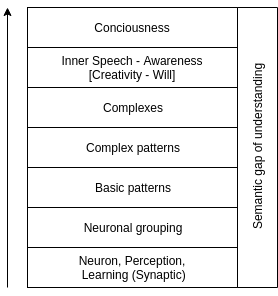
\includegraphics[width=0.4\textwidth]{consciousness_model.png}}
		\caption{Consciousness Model.}
		\label{figure 1}
	\end{figure}

	\subsection{Learning}\label{Le}
	As seen in figure 1, learning builds the very foundation of the model. Without learning, an individual will not be able to achieve consciousness, as the individual will not be able to further group the created connections, thus, will not be able to identify complex or even basic patterns. As no such patterns will be identified, adaptation will not work either, but this will be covered in the next subchapter.

	From a psychological point of view, learning was defined in various ways, e.g. changing the behaviour of an individual in order to survive in its environment but also to develop supporting characteristics based on experience. The act of adapting to new inputs or experience when grouping neurons and identifying patterns can also be considered as learning, as this will put the individual in a different state of behaviour or experience than before. This process of changing its behaviour was a possible definition of learning as well, as described in chapter II.

	Neurologically, learning is intended as making connection between certain neurons, so it is clear that it must be on the ``Learning'' level and on the Neuronal Grouping level of the model shown in figure 1. But this is not true for all kind of learning: as we said in chapter III, the Basal Ganglia is responsible for the procedural memory. But the memories themselves are not born in the Basal Ganglia but in the cortex. After some usage, when the brain realizes the procedural utility of the memory, transfers it to the Ganglia. This process is definitely higher in the consciousness model, probably between Basic Patterns and Complex Patterns.

	\subsection{Adaptation}\label{Ad}
	When talking about adaptation, we described two definitions, (1) adaptation as a verb (the process of adapting) and (2) adaptation as a noun (the outcome). Adaptation definitely lies on a low level of the model. The process of sensitization and desensibilization of the receptors is always done without any consciousness, since a key point of adaptation is the involuntariety of it.


\section{Adaptation and Learning in deep neural networks}

	\subsection{Historical overview of Neural Networks}\label{HONN}
	Starting from the '40, computer and data scientists tangled their work to the concept of learning more and more.
	We find the first contact between the two worlds in 1943 when McCulloch and Pitts modeled a simple neural network to try to explain how neurons might work. \cite{f1}
	This paper is very important because, as McCulloch and Pitts say, for the first time ``Because of the ``all-or-none'' character of nervous activity, neural events and the relations among them can be treated by means of propositional Logic''. From now on, it will be common to shape neural networks according to the human brain in order for them to simulate its behaviour.
	A good example of this idea can be found in ``ADALINE'' and ``MADALINE'', two models developed by Bernard Widrow and Marcian Hoff in 1960 to improve the quality of phone calls. The names are acronyms that stand for (Multiple) ADAptive LINear Elements. The purpose of the first model was to recognize binary patterns from the stream of bits of a phone calls and then predict next bit. MADALINE is a neural network that, using some of the ADALINE's ideas, removes echoes from phone calls. This is thought to be the first application of neural network for a practical problem and it still sees some uses despite being almost sixty years old. \cite{f2}
	Two years later, in 1962, Widrow and Hoff made another important advancement when they developed a learning procedure that allows perceptrons to recognize whether one of them has a big error and then try to adjust it modifying the weights. This way the error gets distributed either across the whole network or to adjacent perceptrons. \cite{f3} This is the base idea behind what now is called backpropagation (that will be discussed further on).

	After a really promising start, though, no significant advancements were made in the following years until in 1975 Fukushima created the first multilayered unsupervised neural network.\cite{f4} From that moment the field flourished again: in 1982 Reilly and Cooper used a multilayer structure where each layer was using a different strategy to solve the problem \cite{f5} and in the same year John Hopfield implemented the first ever bidirectional connection between neurons in a neural network \cite{f6}.

	\subsection{Modern Technologies}\label{MT}
	From this very promising starting point, several new ideas and new technologies have born. We will now explain some of them.

	\begin{itemize}

		\item Perceptron: The basic idea of the perceptron is inspired to the neuron. It is used to decide if a specific input belongs to a class or not. \cite{f7}

		\item Full connected Neural Network: Neural network where all the perceptron of a layer are connected to the perceptron of the next layer;

		\item Backpropagation: As defined by Hecht-Nielsen\cite{f8}, is the process of adjusting the weights of the input nodes of the perceptrons in order to increase he precision of the neural network. Through several iteration the output is compared with the expected result and the weights tweaked, making the model more precise and more reliable while also increasing its generalization;

		\item CNN (Convolutional Neural Network): CNNs are Multilayer Fully Connected Neural Networks. Usually, fully connected neural networks are prone to overfitting data. CNN address this problem combining small and easy patterns to create more complex ones. This is possible because of the hierarchical pattern in data.
		Convolutional networks mimic the way the visual cortex works in animals. Cortical neurons only respond to stimuli coming from a small region of our field of view, but this region is slightly overlapping with the adjacent neurons' ones; \cite{f9}

		\item RNN (Recurrent Neural Network): The connection between nodes forms a directed graph to create a temporal sequence. This allows the network to use its own previous states to extract new knowledge. This particular kind of neural network is commonly used in speech recognition. \cite{f10}

		\item GAN (Generative Adversarial Network): The system is based on two neural networks that play a game where they try to generate new data starting from a training set in such a way that the generated data are similar to the original one. \cite{f11}

	\end{itemize}


\section{Conclusion}

	Overall, research related to learning and adaptation is prominent in many different disciplines, including psychology, neurology and deep learning. A formal definition of both terms can be found in scientific literature, but is very reliant on the research topic and the researchers themselves as they have a different take on the definitions each.

	In chapter II, we looked at and compared different definitions of learning and adaptation in the psychological field of science. In both cases, the definition can either describe it as an activity, the process of changing behaviour or adjusting an individual’s characteristic attributes according to its environment and/or experience, or as the outcome of the process, i.e. adaptation and learning is the state an individual falls into after undergoing changes, adjustments or similar activities.

	Another perspective for defining the terms was covered in chapter III, which covers the neurological context. In order to understand what learning and adaptation mean in neurology, we observed that the process of learning new information and processing it to adapt to changes is very closely related to the concept of memory.

	Psychology and neurology, however,  are not the only research areas were learning and adaptation have an influence on. Further topics in different scientific disciplines were identified in chapter IV:

	\begin{itemize}
		\item Learning Theory: The theory on how humans and non-humans learn.
		\item Educational Studies: Social constructs around students and how they organise, e.g. professional learning groups.
		\item Linguistics: Research on how to learn second language and differences in learning strategies for first and second language.
		\item Computer Science: Different scientific research in the area of mathematics, machine learning and deep learning.
	\end{itemize}

	Based on the insights from the chapters II to IV, we linked the terms to a consciousness model presented within chapter V. Learning and adaptation are very closely related in this context as both are required for building up the neuronal connections needed for the foundation. Furthermore, in order to perform neuronal grouping and identifying basic patterns the process of learning and adaptation is needed as well, creating a loop back to the foundation of the consciousness model.

	With chapter VI, we saw that Learning and adaptation play a major role on Deep Learning and Neural Networks. Perceptrons, Convolution, Backpropagation, ecc are all ideas that come from the attempt of mimicking these very basic processes of the human brain.

	Generally speaking, learning and adaptation are very closely related topics with many different applications and research opportunities in modern science disciplines.

\begin{thebibliography}{00}
%chapter 1
\bibitem{a1} G. M. Stratton (1986), Some preliminary experiments on vision without inversion of the retinal image, University of California

%chapter 2
\bibitem{b1} D. P. Schmitt and J. J. Pilcher (2004), “Evaluating Evidence of Psychological Adaptation: How Do We Know One When We See One?”, in Psychological science, vol. 15, issue 10, pp. 643-649, October 2004.
\bibitem{b2} G. Hall (2003), “The Psychology of Learning”, in Encyclopedia of cognitive science, vol. 2, pp. 837-845.
\bibitem{b3} S. M. Breedlove and N. V. Watson (2013), “Biological Psychology: An Introduction to Behavioral, Cognitive, and Clinical Neuroscience”, 7th edition, Sinauer Associates Inc.
\bibitem{b4} R. A. Rescorla (1988), “Behavioral studies of Pavlovian conditioning”, in Ann. Rev. Neurosci., vol. 11, pp. 329-352.
\bibitem{b5} J. De Houwer (2013), “What is learning? On the nature and merits of a functional definition of learning.”, in Psychonomic Bulletin \& Review, vol. 20, issue 4, pp. 631-642.
\bibitem{b6} A. B. Barron, et al. (2015), “Embracing multiple definitions of learning”, in Trends of Neurosciences, vol. 38, issue 7, pp. 405-407.

%chapter 3
\bibitem{b7} R. Gross (2010), Psychology: The Science of Mind and Behaviour, 6th Edition, Hodder Education, chapter 1
\bibitem{b8} Dougherty, D. P.; Wright, G. A.; Yew, A. C. (2005). Computational model of the cAMP-mediated sensory response and calcium-dependent adaptation in vertebrate olfactory receptor neurons. Proceedings of the National Academy of Sciences. 102 (30): 10415–20.
\bibitem{b9} Chung, S; Li, X; Nelson, S. B. (2002). Short-term depression at thalamocortical synapses contributes to rapid adaptation of cortical sensory responses in vivo. Neuron. 34 (3): 437–46.
\bibitem{b10} Larry R. Squire. The Legacy of Patient H.M. for Neuroscience.
\bibitem{b11} Stocco, Andrea; Lebiere, Christian; Anderson, John R. (2010). Conditional Routing of Information to the Cortex: A Model of the Basal Ganglia's Role in Cognitive Coordination. Psychological Review. 117 (2): 541–74.

%chapter 4
\bibitem{d1} L. Harasim (2012), “Learning Theory and Online Technologies”, Taylor and Francis Group.
\bibitem{d2} R. Baillargeon (1994), “How do infants learn about the physical world?”, in Current Directions in Psychological Science, vol. 3, issue 5, pp. 133-140.
\bibitem{d3} R. DuFour (2004), “What Is a ‘Professional Learning Community’?”, in Educational Leadership, vol. 61, issue 8, pp. 6-10.
\bibitem{d4} S. Gass, et al. (1989), “Linguistic Perspectives on Second Language Acquisition”, Cambridge University Press.
\bibitem{d5} P. Skehan (2003), “A Cognitive Approach to Language Learning”, 5th edition, Oxford University Press.
\bibitem{d6} A. Burns and J. C. Richards (2018), “Learning English as a Second Language”, Camebridge University Press.
\bibitem{d7} W. K. Estes (1950), “Toward a Statistical Theory of Learning”, in Psychological Review, vol. 57, issue 2, pp. 94-107.
\bibitem{d8} S. Shalev-Shwartz and S. Ben-David (2014), “Understanding Machine Learning: From Theory to Algorithms”, Camebridge University Press.


%chapter 5

%chapter 6
\bibitem{f1} W. McCulloch, W. Pitts (1943). ``A logical calculus of the idea immanent in nervous activity'', Bulletin of Mathematical Biophysics, vol. 5, pp. 115-133
\bibitem{f2} B. Widrow and M.E. Hoff, Jr., ``Adaptive Switching Circuits,'' IRE WESCON Convention Record, 4:96-104, August 1960
\bibitem{f3} B. Widrow and M.E. Hoff, ``Associative Storage and Retrieval of Digital Information in Networks of Adaptive `Neurons,''' Biological Prototypes and Synthetic Systems, 1:160, 1962.
\bibitem{f4} Fukushima, K. Biol. Cybernetics (1975) 20: 121. https://doi.org/10.1007/BF00342633
\bibitem{f5} Cooper, L. N. Elbaum, C.Reilly. ``Self organizing general pattern class separator and identifier'', US patent No. 4,326,259, 1982
\bibitem{f6} J. J. Hopfield, ``Neural networks and physical systems with emergent collective computational abilities (associative memory/parallel processing/categorization/content-addressable memory/fail-soft devices)'', Proc. NatL Acad. Sci. USA, Vol. 79, pp. 2554-2558, April 1982
\bibitem{f7}Freund, Y.; Schapire, R. E. (1999). ``Large margin classification using the perceptron algorithm'' (PDF). Machine Learning. 37 (3): 277–296. doi:10.1023/A:1007662407062.
\bibitem{f8} R. Hecht-Nielsen, ``Neural Networks for Perception'', Chapter 3, ``Theory of the Backpropagation Neural Network'' by Robert Hecht-Nielsen, Proceedings of the International Joint Conference on Neural Networks 1, 593–611, June 1989
\bibitem{f9} Fukushima, K. (2007). ``Neocognitron''. Scholarpedia. 2 (1): 1717. doi:10.4249/scholarpedia.1717.
\bibitem{f10} H. Sak, A. Senior, F. Beaufays (2014). ``Long Short-Term Memory recurrent neural network architectures for large scale acoustic modeling'', In INTERSPEECH-2014, 338-342
\bibitem{f11} I. J. Goodfellow, J. Pouget-Abadie, M. Mirza, B. Xu, D. Warde-Farley, S. Ozair, A. Courville, Y. Bengio, (2014) Generative Adversarial Nets.

%chapter 7

\end{thebibliography}
\vspace{12pt}

\end{document}
